\documentclass[10pt,letterpaper]{article}
\usepackage[utf8x]{inputenc}
\usepackage{amsmath}
\usepackage{amsfonts}
\usepackage{amssymb}
\usepackage{graphicx}
\usepackage{lmodern}
\usepackage[hidelinks]{hyperref}
\usepackage{pgf}
\usepackage{pgfplots}
\usepackage{tabularx}
\pgfplotsset{compat=1.16}
\usepackage[american, nooldvoltagedirection, siunitx, americanvoltages]{circuitikz}
\usetikzlibrary{fit}

\usepackage[
type={CC},
modifier={by-sa},
version={4.0},
]{doclicense}

%\usepackage[left=2cm,right=2cm,top=2cm,bottom=2cm]{geometry}
\author{Scott Howard (KD9PDP)}
\date{}
\title{\footnotetext{\doclicenseThis} Search for the Minimalist QRP Class E Amplifier Filter Typology}
\begin{document}
\maketitle

\section*{Quick Summary: Do this!}
Use a Pi-networks with second-harmonic notch filter, as seen in Figure \ref{figminipinotch} and design equations are below and shown in Section \ref{section2ndorder}. Alternatively, you can use a T-network with a second-harmonic notch filter with similar results. You can to trade off power and efficiency a little bit as you see fit: see Table \ref{comparetable} for a comparison.

\begin{figure}[h]
\centering
\begin{circuitikz}[scale=0.75, transform shape]
\draw
(2,0) node[nigfetd](fet){}
(fet.D) -- (2,1) to[short,] (2,1) to[short] (3,1) to[L=$L_1$, *-] (3,3)
  node[vcc](VCC){$V_{CC}$};
  \draw (fet.S) -- (2,-1) node[ground]{};
  \draw (fet.G) to[sqV] (fet.G -| 0,-2) -| (0,-1)
  node[ground]{};
  \draw (3,1) to[C=$C_1$] (3,-1) node[ground]{};
  \draw (3,1) to[C=$C_f$,]
  (5,1) to[L=$L_{tot}$, name=Lf]
  (7,1) to[C=$C_2$]
  (7,-1) node[tlground]{};
  \draw  (7,1) to[L, l_=$L_2$,*-*] (9,1) to[C=$C_3$] (9,-1) node[tlground]{};
  \draw (9,1)--(10.5,1)
  to[R=$R_{ant}$] (10.5,-1) node[tlground]{};
  \draw (7,1) -- (7,2) to[C=$C_4$] (9,2) -- (9,1);
\end{circuitikz}
\caption{Class E amplifier with pi-network with second harmonic notch}\label{figminipinotch}
\end{figure}

David Cripes (NM0S) was the first to promote this typology, and there is a great design spreadsheet based on it. The design equations presented here are a little different, provide more flexibility, and yield slightly higher efficiencies for the same output power (e.g., 89\% vs 85\% at 3 W output).


\subsection*{Design Procedure}
This is a minimalist, easy version of Section \ref{section2ndorder}.
\begin{enumerate}
\item Pick a desired output power. You'll be practically limited by thermal effects. Based on SPICE simulations, for $V_{CC}=\SI{12}{\volt}$ with 3 parallel BS170 transistors, desired output power should be less than 4 W. Find the value for the apparent load resistance and the corresponding circuit $Q$s:
\begin{align*}
R_L&=0.58\frac{V_{CC}^2}{P_{out}} &
Q&=3+\sqrt{\frac{R_L}{5}-1} 
\end{align*}
%
%\begin{table}
%\centering
%\begin{tabular}{c|c|c|c|c|c|c|c|c}
%$R_L$ $(\Omega)$ & 15 & 20 & 25& 30 & 35 & 40 &45 & 50 \\ \hline
%$R_v$  $(\Omega)$& 4.07 & 4.56 & 5.00 & 5.42 & 5.81 & 6.18 & 6.55 & 6.90\\
%\end{tabular}
%\caption{Virtual $R_v$ for a corresponding $R_L$ for a 50 $\Omega$ antenna and design $Q=5$.}\label{rvtable}
%\end{table}


\item Find all the component values:
\begin{align*}
C_1&=\frac{1}{5.4466 \omega R_L} & L_1&\gg 2.84\frac{R_L}{\omega} \\
C_f&=\frac{1}{Q\omega R_L} &
L_{tot}&=(Q+1.1525)\frac{R_L}{\omega} \\
C_2&=\frac{(Q-3)R_L}{\omega} &
C_3&=\frac{150}{\omega}\\
L_2&=\frac{15 Q }{4\omega} &
C_4 &= \frac{1}{15 Q \omega}
\end{align*}
\end{enumerate}
\subsubsection*{How did we get the simplified equations?}
The simplification comes from taking the equations in Section \ref{section2ndorder} for a $\SI{50}{\ohm}$ antenna, then setting $R_v=5$ and solving the equations. It's perfectly valid and rigorous to just set $R_v=5$, there are no approximations made. $R_v=5$ corresponds to choosing a $Q\approx 5$ for all $R_L$ from 15 to 50 $\Omega$. Since we're free to choose any $Q$ we want (granted we achieve the required harmonic suppression, which we do) it's valid!

\newpage
\section{Intro}

Class E power amplifiers are popular for use in QRP transmitters because of they achieve high efficiency ($>90\%$) using relatively common and inexpensive components. While there's a lot of info out there about Class E theory and design, there hasn't been many comparative reviews of the different approaches to building a Class E amplifier. Understanding the approaches can better guide balancing complexity and performance, as well as make sure \textit{incompatible} filters are not used. While tempting, adding on a filter you are comfortable with to the output of a Class E amplifier might be incompatible with the design typologies, so hopefully this analysis can help prevent those issues while also determining what is minimally required for a good QRP Class E design.

First, this paper will show a comparison of the different general typologies in Section \ref{overview}. As a reference, a theoretically derivation of the standard design equations is given in Section \ref{standarddesign}. A companion paper looks at the QCX Class E design, a unique design that's fundamentally different than the standard designs, but requires more components to achieve similar efficiency. It's important to mention because QCX Class E is fundamentally incompatible with ``standard" design typologies and filters.

\section{Overview of Typologies}\label{overview}

Nearly all amateur radio QRP Class E amplifiers look like Figure \ref{ClassEnocurrents}. Some square wave signal modulates the gate of a MOSFET. The drain is biased through an inductor $L_1$ and connected to ground through $C_1$. Gate modulation causes voltage modulation at the drain. Filters are used to extract the RF signal you would like to apply to your load resistor $R_L$ (i.e., your antenna).


\begin{figure}
\centering
\begin{circuitikz}
\draw
(0,0) node[nigfetd](fet){}
(fet.D) -- (0,1) to[short,] (1,1) to[short] (3,1) to[L=$L_1$, *-] (3,3)
  node[vcc](VCC){$V_{CC}$};
  \draw (3,1) node[below]{$v_c$};
  \draw (fet.S) -- (0,-1) node[ground]{};
  \draw (fet.G) to[sqV] (fet.G -| -2,-2) -| (-2,-1)
  node[ground]{};
  \draw (1,1) to[C=$C_1$] (1,-1) node[ground]{};
  \draw (3,1) to[short] (4,1)
  to[bandpass, l=Filter, name=filter] (6,1) -- (7,1) to[R=$R_L$, name=RL] (7,-1)
  node[ground](gnd){};
  \node[rectangle, draw, dashed, fit=(RL) (filter) (filterlabel) (RLlabel) (gnd)](box){};
  \node [above] at (box.north) {Typology Specific};
\end{circuitikz}
\caption{Generic Class E Amplifier}
\label{ClassEnocurrents}
\end{figure}

The design choices therefore become:
\begin{itemize}
\item What value should I choose for $L_1$?
\item What value should I choose for $C_1$?
\item What filter should I use?
\begin{itemize}
\item How much filtering do I need to do? (The FCC requires that the average power of spurious emissions are at least 43 dB below the fundamental frequency. FCC 97.307d.)
\item What complex impedance should the filter present? (required for high efficiency operation)
\item Do I need my filter to do any impedance matching or impedance transformation on $R_L$ to transmit at a desired power level?
\end{itemize}
\item Other typologies: There (literally) an infinite number of other types. However, DIY QRP transmitters tend to keep it simple. For example, amplifiers with shunt capacitors and shunt filters can work too.
\end{itemize}

There are several strategies to answer the above questions. These strategies can be broken down as follows:

\begin{itemize}
\item `\textbf{`Standard" Designs}, the most common in QRP and homebrew devices. Mostly based on Nathan Sokal's (WA1HQC) 2001 QEX article. A large RF choke is used for $L_1$. The ``standard" design equations are derived in Section \ref{standarddesign} where we'll find:
\begin{align*}
C_1 &= \frac{1}{5.4466\omega R_L} &L_1 &\gg \frac{2.84 R_L}{\omega}
\end{align*}
as a note, above shows a the results of a new derivation  and approach for finding the limit for what to make $L_1$. This design has the following filter \textit{requirements}: infinite impedance at DC and all frequencies except the fundamental frequency. The filter should present a specific complex inductive load at the fundamental frequency. There are several approaches to developing appropriate filters that we will explore:
\begin{itemize}
\item A standard LC series bandpass filter.
\item An LC bandpass filter in series with an L impedance matching low-pass filter to achieve higher output power.
\item An LC bandpass filter placed in series with a Pi or T impedance matching low-pass filter. This achieves improved harmonic suppression and higher output power.
\item An LC bandpass filter in series with a Pi or Timpedance matching low-pass filter that utilizes a notch filter to essentially eliminate the second harmonic spurious emission and achieving higher output power. This was first shown to be effective by David Cripe (NM0S) and described in his ``Class E Power Amplifiers for QRP" paper.
\end{itemize}
\item \textbf{``QCX Class E."} This design is used in the QCX QRP transceiver\footnote{\url{https://qrp-labs.com}}. The QCX design equations are derived in the complimentary document:
\begin{align*}
L_1&=\frac{3 \pi R_L Z(2\omega) }{[2R_L+8Z(2\omega)]\omega}
& C_1&=\frac{1}{L_1 (2\omega)^2}
\end{align*}
Where $Z(2\omega)$ is the entirely real impedance at $2\omega$. This design has the following filter \textit{requirements}: infinite impedance at DC, purely real (resistive) at the fundamental frequency, purely restive (or large) at the second harmonic, capacitive at all other harmonics. So far, only one filter typology has been used, seen in Figure \ref{ClassEqcx}.
\end{itemize}

The design equations for all the above are derived in the following sections. We can use those equations in SPICE models to simulate performance. Ngspice was used to evaluate each of the above typologies to compare what is needed for a minimal QRP transmitter, the results are presented in Table \ref{comparetable}. Increased complexity filter yields both higher harmonic suppression and smaller inductors. The simplest amplifier typology to reach FCC requirements is a Pi-network, and both Pi- and T-networks are appropriate when combined with a second harmonic notch filter. The following sections explore all of this in more detail.




\begin{table}
\centering
%\begin{tabularx}{0.9\textwidth}{cc|ccc}
\begin{tabular}{ccc|ccccc}
 &  & &  &  & \textbf{Spur. Rej./} & &  \\
\textbf{Type} & $R_L$ &$Q$ & \textbf{Max.} $L$ & \textbf{\#} $L$ & \textbf{Notch} & $\left\langle P_{out}\right\rangle$ & $\eta$ \\
\hline
\hline 
%Std. & & 10 & $\SI{13}{\micro\henry}$ & 27 dB & 1.5 W & 94\%\\
Std. & 50 & 20 & $\SI{24}{\micro\henry}$ & 1 & 32 dB & 1.5 W & 94\%\\ \hline 
L-match & 10 & 20 & $\SI{5}{\micro\henry}$ & 1 & 40 dB & 4.0 W & 63\%\\ \hline 
L-match & 15 & 20 & $\SI{7}{\micro\henry}$ & 1 & 37 dB & 4.0 W & 80\%\\ \hline 
%L-match & 10 & 30 & $\SI{7}{\micro\henry}$ & 43 dB & 4.0 W & 64\%\\
L-match & 20 & 20 & $\SI{10}{\micro\henry}$ & 1 & 37 dB & 3.3 W & 86\%\\ \hline 
L-match & 25 & 20 & $\SI{18}{\micro\henry}$ & 1 & 36 dB & 2.8 W & 89\%\\ \hline 
%Pi-match & 10 & 10 & $\SI{2.5}{\micro\henry}$ & \textbf{63 dB} & 4.0 W & 63\%\\
%Pi-match & 15 & 10 & $\SI{3.7}{\micro\henry}$ & \textbf{61 dB} & 4.1 W & 81\%\\
%Pi-match & 20 & 10 & $\SI{5.0}{\micro\henry}$ & \textbf{61 dB} & 3.4 W & 86\%\\
%Pi-match & 25 & 10 & $\SI{6.2}{\micro\henry}$ & \textbf{61 dB} & 2.9 W & 89\%\\
Pi-match & 10 & 5 & $\SI{1.4}{\micro\henry}$ & 2 & \textbf{49/70 dB} & 4.1 W & 63\%\\ \hline 
Pi-match & 15 & 5 & $\SI{2.1}{\micro\henry}$ & 2 & \textbf{48/70 dB} & 4.2 W & 81\%\\ \hline 
Pi-match & 20 & 5 & $\SI{2.8}{\micro\henry}$ & 2 & \textbf{48/70 dB} & 3.5 W & 86\%\\ \hline 
Pi-match & 25 & 5 & $\SI{3.4}{\micro\henry}$ & 2 & \textbf{48/70 dB} & 3.0 W & 89\%\\ \hline
Pi-match & 50 & 5 & $\SI{6.9}{\micro\henry}$ & 2 & \textbf{49/70 dB} & 1.6 W & 94\%\\ \hline 
T-match & 10 & 5 & $\SI{2.2}{\micro\henry}$ & 2 & 34/\textbf{54 dB} & 3.6 W & 83\%\\ \hline 
T-match & 15 & 5 & $\SI{3.2}{\micro\henry}$ & 2 & 36/\textbf{56 dB} & 2.8 W & 87\%\\ \hline 
T-match & 20 & 5 & $\SI{4.2}{\micro\henry}$ & 2 & 38/\textbf{58 dB} & 2.4 W & 89\%\\ \hline 
T-match & 25 & 5 & $\SI{5.1}{\micro\henry}$ & 2 & 39/\textbf{59 dB} & 2.1 W & 91\%\\ \hline
T-match & 50 & 5 & $\SI{9.7}{\micro\henry}$ & 2 & 40/\textbf{60 dB} & 1.6 W & 94\%\\ \hline 
QCX & 50 &  & $\SI{1.7}{\micro\henry}$ & 3+1 & \textbf{45 dB} & 3.4 W & 85\%\\ \hline 
NM0S Notch &  &  & $\SI{1.1}{\micro\henry}$ & 2 & \textbf{57 dB} & 3.0 W & 85\%\\ \hline
NM0S Notch &  &  & $\SI{0.7}{\micro\henry}$ & 2 & \textbf{57 dB} & 4.0 W & 75\%\\ \hline 
\end{tabular}
\caption{ngSpice models of Class E amplifiers (using 3 parallel BS170 transistors). $f=\SI{7.1}{\mega\hertz}$ $V_{CC}=\SI{12}{\volt}$, $R_{ant}=\SI{50}{\ohm}$. Max $L$ is largest inductor value (excluding choke inductor) and ``\# $L$" is the number of inductors in the filter (QCX has a +1 because the feed inductor is also frequency dependent and acts as part of the filter). Spurious rejection is given without and with ``notch" filters (see text). $Q<20$ for required bandwidth.}\label{comparetable}
\end{table}



\subsection{Standard/Traditional Class E}

The standard Class E is given in Figure \ref{ClassEtradfiltmatchsimple}. A simple series LC bandpass filter performs both filtering and impedance matching (see Section \ref{standarddesign} for derivations). However the filter must be very high ($Q>40$) to reach the 43~dB of harmonic filtering required, and therefore is not seen in QRP transmitters. However, this model gives us the starting point to improve performance since it gives us the general things we we want: (a) a high impedance at all frequencies except our designed fundamental frequency $\omega$ (green line in Figure \ref{ClassEtradfiltmatchsimple}) and (b) some harmonic attenuation . We need 43~dB (red line in Figure \ref{ClassEtradfiltmatchsimple}), and since Class Es naturally have 5.7~dB harmonic suppression, our filter should at least suppress $\approx 37.3$~dB (dotted red line) at the second harmonic (dashed green line).



\begin{figure}
\centering
\begin{circuitikz}
  \draw (1,1) node[left]{$v_c$} to[C=$C_f$,o-]
  (3,1) to[L=$L_{f}$, name=Lf]
  (5,1) to[L=$\Delta L$, name=deltaL]
  (7,1) to[R=$R_{ant}$]
  (7,-1) node[tlground]{};
  \node[rectangle, draw, dashed, fit=(Lf) (deltaL) (Lflabel) (deltaLlabel)](box){};
  \node[above] at (box.north){$L_{tot}$};
\end{circuitikz}
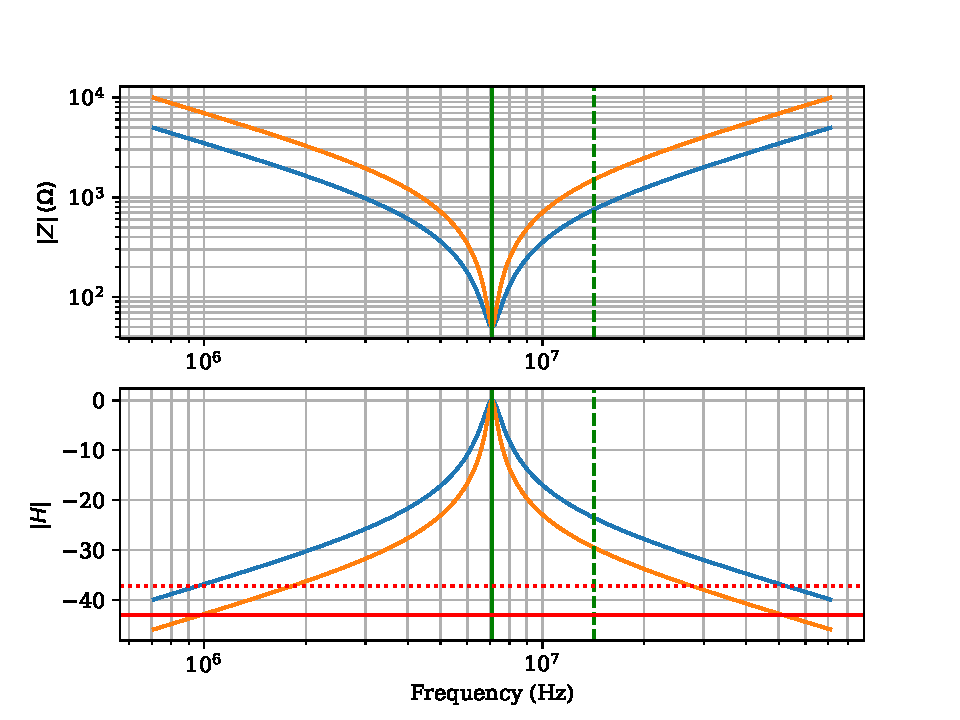
\includegraphics[width=.8\textwidth]{LCbp.pdf}
\caption{Traditional LC bandpass filter for a Class E Amplifier for $Q=10$ (blue) and $Q=20$ (orange). Fundamental frequency is 7.1 MHz (green line), second harmonic at 14.2 MHz (dotted green line) are shown as vertical lines. FCC required attenuation of 43 dB (red line) and the target minimum harmonic suppression including Class E natural suppression of 5.7 dB (dotted red line). }
\label{ClassEtradfiltmatchsimple}
\end{figure}


The component parameters for a desired bandwidth ($Q_f=\frac{f}{\Delta f}$) when the load resistance is equal to the antenna resistance $R_L=R_{ant}$ can be found using:
\begin{align*}
C_f &=\frac{1}{Q_f R_L \omega} &
L_{tot} & =\frac{R_L}{\omega}\left(Q_f+1.1525\right)
\end{align*}
Generally, $R$ is the real resistance of the load seen at the MOSFET drain  (i.e., the resistance $R_L$ after the LC transformers in the sections below).

Sokal has a famous QEX paper that addresses Class E amplifiers with finite $Q$s. Basically, if your impedance at harmonics is not infinity, your can't have the ideal, theoretical 100\% efficiency. An intersting note is that when the paper was written, QRP transmitters only needed 30 dB of harmonic suppression, so $Q=20$ would work. The larger suppression requirements now require more complicated filters, which causes the equations to be a little bit different.

\subsubsection{``Power Boost" Class E}
As we'll see in Section \ref{standarddesign}, you can increase the output power by increasing $V_{CC}$ or decreasing the load resistance. We can use an impedance matching LC circuit to decrease the load resistance, thereby boosting power (and doing some low-pass-filtering along the way).

To increase output power and perform additional low-pass filtering, you can use an LC impedance transformer before the antenna. This lowers $R_L<R_{ant}$, and does not require an additional inductor since you can add the transformer inductor inductance to the existing inductor. The circuit is presented in Figure \ref{ClassEimptrans1}.

\begin{figure}
\centering
\begin{circuitikz}
  \draw (1,1) node[left]{$v_c$} to[C=$C_f$,o-]
  (3,1) to[L=$L_{tot}$, name=Ltot]
  (5,1) to[L=$L_{match}$, name=Lm]
  (7,1) to[C=$C_2$]
  (7,-1) node[tlground]{};
  \draw  (7,1) -- (8.5,1)  to[R=$R_{ant}$]
  (8.5,-1) node[tlground]{};
  \node[rectangle, draw, dashed, fit=(Lm) (Ltot) (Lmlabel) (Ltotlabel)](box){};
  \node[above] at (box.north){$L_2$};
\end{circuitikz}
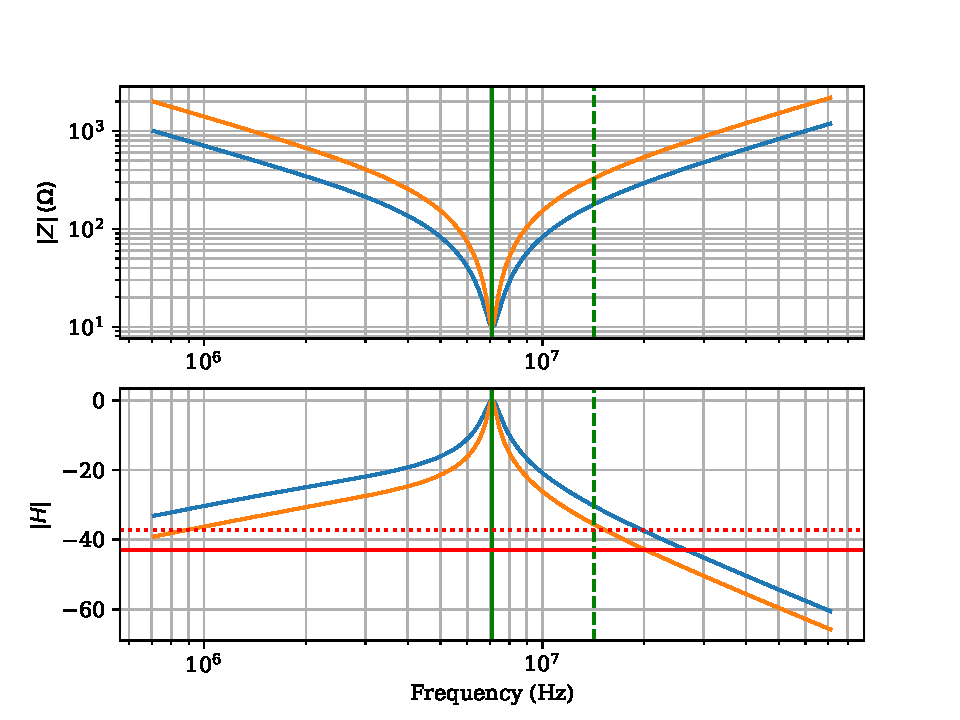
\includegraphics[width=.8\textwidth]{LCbpimp1.pdf}
\caption{``Power Boosting" Impedance Transformer Class E with BPF. Both the transformer and BPF have the same $Q$: $Q=10$ (blue) and $Q=20$ (orange). $H$ is normalized to $1$ at $\omega$.}
\label{ClassEimptrans1}
\end{figure}

First, determine how much power out ($P_{out}$) you'd like. From there you can find $C_2$ and $L_{match}$ usint a standard L-match circuit:

\begin{align*}
R_L&=\frac{0.58V_{CC}^2}{P_{out}}
& Q &= \sqrt{\frac{R_{ant}}{R_L}-1}  \\
%=\sqrt{\frac{R_{ant}{P_{out}}}{0.58V_{CC}^2}-1}\\
L_{match}&=\frac{Q R_L}{\omega} & C_2&=\frac{Q}{R_{ant} \omega}
\end{align*}

Practically speaking, the load resistance should be at least $R_L>\SI{10}{\ohm}$ as to not draw too much current and avoid excessively large voltages on the filter components. Therefore, $1<Q<2$ and $P_{new}<5\times P_{orig}$. Figure \ref{ClassEimptrans1} shows that using a L-match $Q=2$, corresponding to $5\times$ higher output power with a BPF $Q=20$ gets really close to hitting the FCC requirements. However, that requires a $\SI{22}{\micro\henry}$ inductor, which is quite large. But it's possible!

\subsubsection{Second Order ``Power Boosting" Impedance Transforming}\label{section2ndorder}

If a simple L-network impedance transform doesn't get enough harmonic suppression, you can further boost the $Q$ of the low-pass filter by using a ``pi" or ``t" network. Circuit examples are given in Figure \ref{ClassEimptrans2}. 


\begin{figure}
\centering
\begin{circuitikz}
  \draw (3,1) node[left]{$v_c$} to[C=$C_f$,o-]
  (4.5,1) to[L=$L_{tot}$, name=Lf]
  (7,1) to[C=$C_2$,name=C2]
  (7,-1) node[tlground](gnd1){};
  \draw  (7,1) to[L=$L_2$, name=L2] (9,1) to[C=$C_3$,name=C3] (9,-1) node[tlground](gnd2){};
  \draw (9,1)--(10.5,1)
  to[R=$R_{ant}$] (10.5,-1) node[tlground]{};
  \node[rectangle, draw, dashed, fit=(C2) (gnd1) (gnd2) (L2) (L2label) (C3label) (C3)](box){};
  \node[above] at (box.north){Pi Network};
\end{circuitikz}
\begin{circuitikz}
  \draw (3,1) node[left]{$v_c$} to[C=$C_f$,o-]
  (4.5,1) to[L=$L_{tot}$, name=Lf]
  (7,1) to[L=$L_2$, name=L2] (9,1) to[C=$C_2$,name=C3] (9,-1) node[tlground](gnd2){};
  \draw (9,1) to[L=$L_3$, name=L3]
  (11,1) to[R=$R_{ant}$] (11,-1) node[tlground]{};
  \node[rectangle, draw, dashed, fit=(C2) (gnd1) (gnd2) (L2) (L2label) (L3label) (L3)](box){};
  \node[above] at (box.north){Tee Network};
  \node[rectangle, draw, dotted, fit =(Lf) (Lflabel) (L2) (L2label)](box2){};
\end{circuitikz}
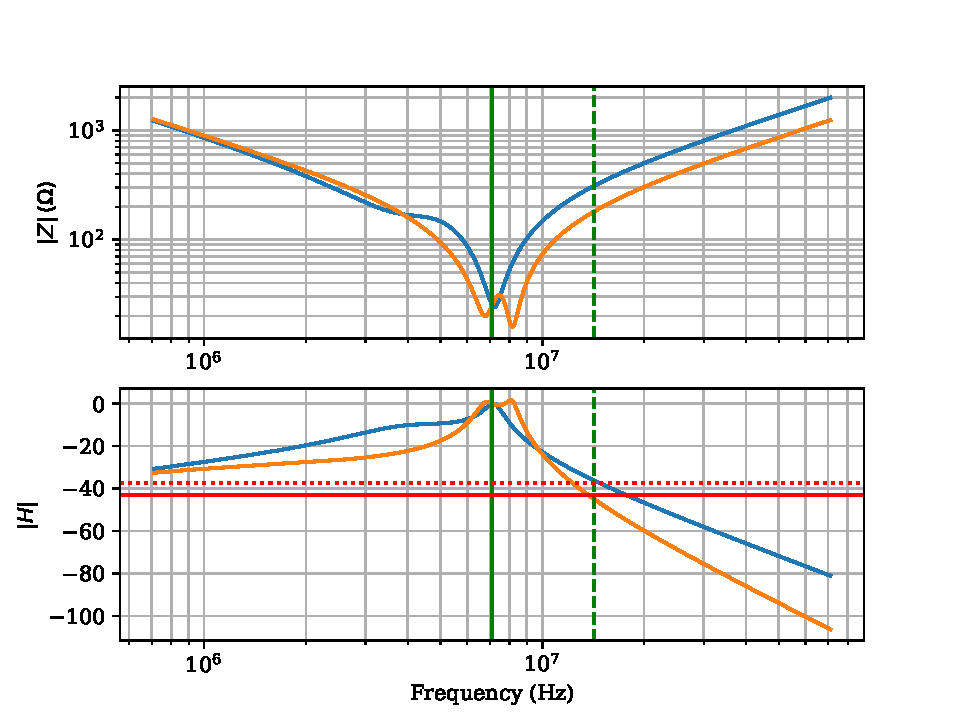
\includegraphics[width=0.8\textwidth]{LCbpimp2.pdf}
\caption{Second Order ``Power Boosting" Impedance Transformer Class E, each with a $Q=5$ and $R_L=\SI{25}{\ohm}$. T-network in blue, pi-network in orange.}
\label{ClassEimptrans2}
\end{figure}

Both configurations are low-pass filters that can be designed to make the load appear real and smaller than $R_{ant}$, thereby boosting power. The performance of the two are comparable, with T-networks having a slight edge in efficiency and Pi-networks have an edge in harmonic suppression.

The following sections shows how to calculate the values for each network.

\subsubsection{Pi Matching}
The pi network component values are calculated as follows:
\begin{enumerate}
\item Choose a $Q$ that meets your bandwidth need. Lower $Q$ means smaller inductors, and a $Q=5$ seems to work pretty well.
\item Find your desired apparent load resistance using $R_L=\frac{0.58 V_{CC}^2}{P_{out}}$
\item Find the value of a virtual resistance $R_v$ that will each side of the pi-network will appear as:
\begin{align*}
Q&=\sqrt{\frac{R_L}{R_v}-1}+\sqrt{\frac{R_{ant}}{R_v}-1}\approx \sqrt{\frac{R_v}{R_L}-1}\\
R_v&\approx \frac{R_{ant}}{(Q^2+1)}
\end{align*}
If you can use a computer to solve the un-approximated version, great - but the approximate one works OK too.
\item Find the $Q$s corresponding to each side of the pi-network:
\begin{align*}
Q_1 & = \sqrt{\frac{R_L}{R_v}-1} &Q_2 &=\sqrt{\frac{R_{ant}}{R_v}-1}
\end{align*}
\item Find $C_2$, $C_3$, and $L_2$:
\begin{align*}
C_2 &= \frac{Q_1 R_L}{\omega } &C_3 &= \frac{Q_2 R_{ant}}{\omega } & L_2 = \frac{R_v}{\omega} (Q_1+Q_2)
\end{align*}
\end{enumerate}

\subsubsection{T-Matching}: The tee network component values are calculated as follows:
\begin{enumerate}
\item Choose a $Q$ that meets your bandwidth need
\item Find your desired apparent load resistance using $R_L=\frac{0.58 V_{CC}^2}{P_{out}}$
\item Find the value of a virtual resistance $R_v$ that will each side of the t-network will appear as:
\begin{align*}
Q&=\sqrt{\frac{R_v}{R_L}-1}+\sqrt{\frac{R_v}{R_{ant}}-1}\approx \sqrt{\frac{R_v}{R_L}-1}\\
R_v&\approx R_L(Q^2+1)
\end{align*}
Again, use a computer to solve this if you can, but the approximation is OK too.
\item Find the $Q$s corresponding to each side of the t-network:
\begin{align*}
Q_1 & = \sqrt{\frac{R_v}{R_L}-1} &Q_2 &=\sqrt{\frac{R_v}{R_{ant}}-1}
\end{align*}
\item Find $L_2$,  $L_3$, and $C_2$
\begin{align*}
L_2 &= \frac{Q_1R_L}{\omega} &L_3 &= \frac{Q_2R_{ant}}{\omega} & C_2 = \frac{1}{R_v\omega}(Q_1+Q_2)
\end{align*}
\end{enumerate}



\subsection{Pi- and T-Networks with Second Harmonic Notch Filters}

To ensure that the second harmonic is properly suppressed (and impedance is zero), you can add capacitors in parallel to $L_2$ in a pi network or parallel to $L_3$ in a t network. This parallel LC branch can be tuned to $2\times \omega$ to eliminate the second harmonic. This is illustrated in Figure \ref{ClassEimpnotch}. Now both typologies reach the desired harmonic suppression levels. \textbf{\textit{We've found designs suitable for easy QRP transmitters!}}

Since Pi-networks seem the most promising, here's the design equation for $L_2$ and $C_4$ (in Pi) or $L_3$ and $C_3$ (in T):
\begin{align*}
L_{new}&=\frac{3}{4}L_{orig} &
C=\frac{1}{(2\omega)^2L_{new}}
\end{align*}
where $L_{orig}$ is what the inductor would be following the standard Pi- or T-network design.

There we have it! These work great - but you still need to keep the $Q>5$. Even though you are suppressing $2\omega$, any $Q<5$ will result in having too much spurious $3\omega$ emission.

\begin{figure}
\centering
\begin{circuitikz}
  \draw (3,1) node[left]{$v_c$} to[C=$C_f$,o-]
  (5,1) to[L=$L_{tot}$, name=Lf]
  (7,1) to[C=$C_2$]
  (7,-1) node[tlground]{};
  \draw  (7,1) to[L, l_=$L_2$] (9,1) to[C=$C_3$] (9,-1) node[tlground]{};
  \draw (9,1)--(10.5,1)
  to[R=$R_{ant}$] (10.5,-1) node[tlground]{};
  \draw (7,1) -- (7,2) to[C=$C_4$] (9,2) -- (9,1);
\end{circuitikz}
\begin{circuitikz}
  \draw (3,1) node[left]{$v_c$} to[C=$C_f$,o-]
  (4.5,1) to[L=$L_{tot}$, name=Lf]
  (7,1) to[L=$L_2$, name=L2] (9,1) to[C=$C_2$,name=C3] (9,-1) node[tlground](gnd2){};
  \draw (9,1) to[L, l_=$L_3$, name=L3]
  (11,1) to[R=$R_{ant}$] (11,-1) node[tlground]{}
  (9,1) -- (9,2) to[C=$C_3$] (11,2) -- (11,1);
  \node[rectangle, draw, dotted, fit =(Lf) (Lflabel) (L2) (L2label)](box2){};
  \node[above] at (box2.north) {$L_{tot'}$};
\end{circuitikz}
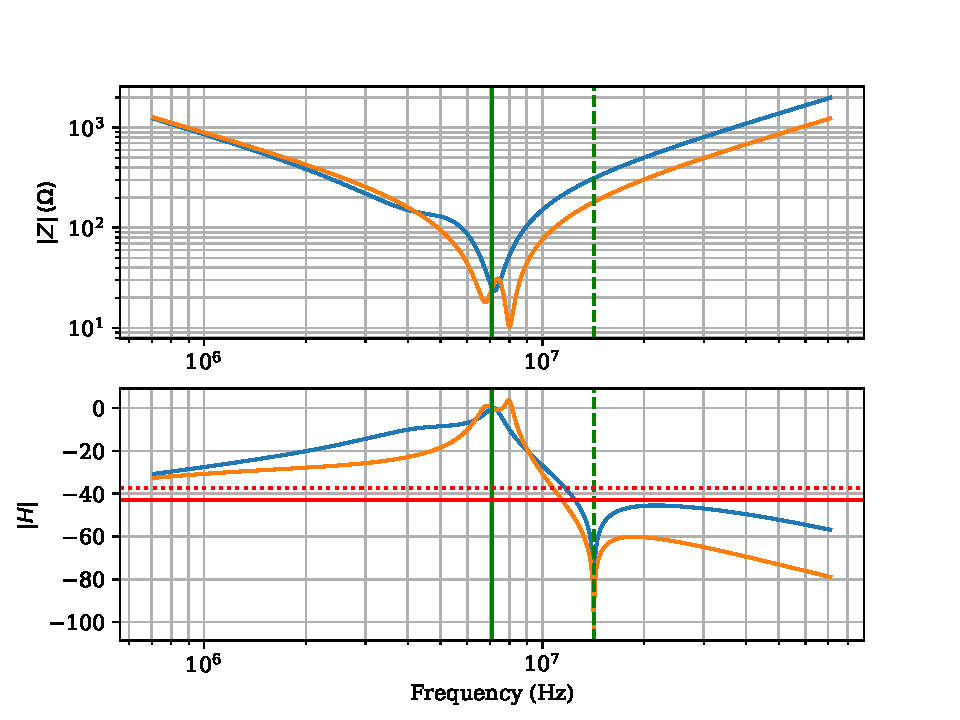
\includegraphics[width=.8\textwidth]{LCbpimp3.pdf}
\caption{Notch Second Harmonic Pi- and T-Network Impedance Transformer Class E. T-network is blue, Pi-network is orange. Both with a $Q=5$ and $R_L=\SI{25}{\ohm}$.}
\label{ClassEimpnotch}
\end{figure}





\subsection{QCX Class E}
Finally we arrive at the QCX Class E. This actually is a completely different design and derivation (see the other document for QCX analysis). The standard equations don't hold because this entire design is based on not needing extra inductance to impedance match to $R_{ant}$, thereby simplifying the design since you can use off-the-shelf, well-known, broadband (low $Q$), completely real impedance matching filters. In fact, adding extra inductance (as required in ``normal" class E amplifiers) will \textbf{\textit{hurt}} QCX Class E performance. The schematic is presented in Figure \ref{ClassEqcx}.


\begin{figure}
\centering
\begin{circuitikz}
  \draw (3,1) node[left]{$v_c$} to[C=$C_f$,o-]
  (5,1) to[L=$L_2$, name=Lf]
  (7,1) to[C=$C_3$]
  (7,-1) node[tlground]{};
  \draw  (7,1) to[L=$L_3$] (9,1) to[C=$C_4$] (9,-1) node[tlground]{};
  \draw (9,1) to [L=$L_4$] (11,1) 
  to[C=$C_5$] (11,-1) node[tlground]{};
  \draw (11,1) -- (12.5,1) to[R=$R_{ant}$] (12.5,-1) node[tlground]{};
  \draw (5,1) to[C=$C_2$] (5,-1) node[tlground]{};
\end{circuitikz}
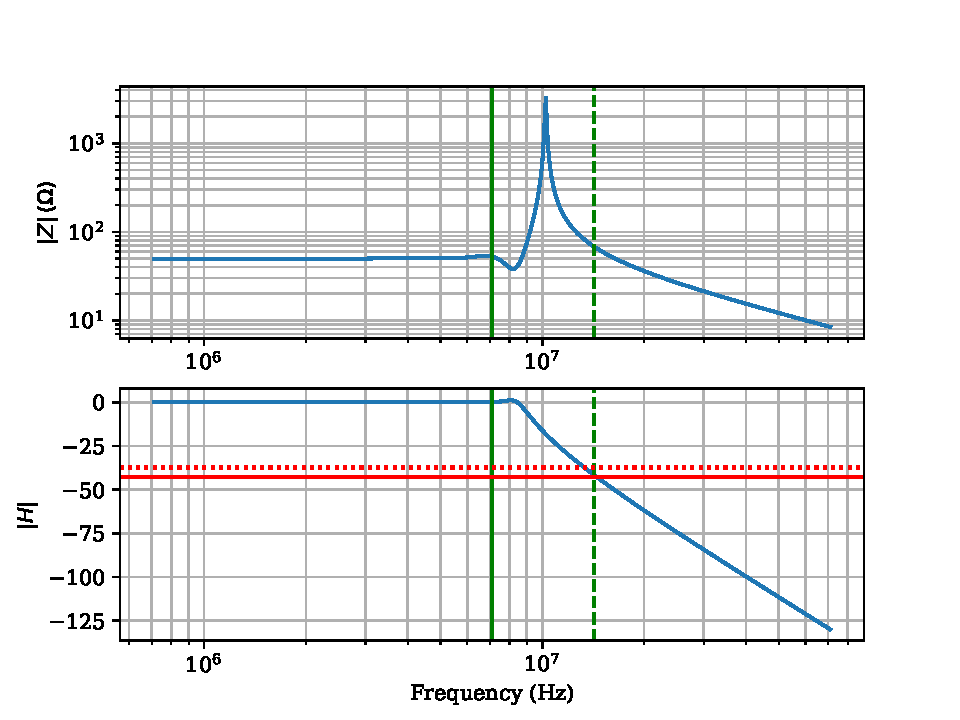
\includegraphics[width=.8\textwidth]{QCXfilt.pdf}
\caption{QCX Completely-Real LPF Class E}
\label{ClassEqcx}
\end{figure}




\section{Traditional Class E Amplifiers}\label{standarddesign}

\begin{figure}
\centering
\begin{circuitikz}
\draw
(0,0) node[nigfetd](fet){}
(fet.D) -- (0,1) to[short, i<=$i_t$] (1,1) to[short, i<=$i_s$] (3,1) to[L=$L_1$, i<=$i_l$] (3,3)
  node[vcc](VCC){$V_{CC}$};
  \draw (fet.S) -- (0,-1) node[ground]{};
  \draw (fet.G) to[sqV] (fet.G -| -2,-2) -| (-2,-1)
  node[ground]{};
  \draw (1,1) to[C=$C_1$, i=$i_c$, v=$v_c$] (1,-1) node[ground]{};
  \draw (3,1) to[short, i_=$i_{load}$] (4,1)
  to[bandpass, l=Filter] (6,1) -- (7,1) to[R=$R_L$, v=$v_r$] (7,-1)
  node[ground]{};
\end{circuitikz}
\caption{Generic Class E Amplifier}
\label{ClassE}
\end{figure}

All Class E amplifiers generally have the same structure (with a few exceptions), shown in \ref{ClassE}. The basic structure consists of:
\begin{itemize}
\item A MOSFET is switched on and off by a pulsed voltage source applied to its gate. The fluctuating switch causes the voltage $v_c$ to fluctuate, and current to flow through $i_l$, $i_c$, and $i_{load}$.
\begin{itemize}
\item When the switch is closed: current flows through $i_t$ and and voltage at the node connected the filter, $L_1$, $C_1$, and transistor drain is grounded (i.e., $v_c=0$).
\item When the switch is open: no current flows through the transistor should be close to zero ($i_t=0$)
\end{itemize}
\item A filter is placed such that $V_r$ is purely a single harmonic. The FCC requires 43 dB suppression of higher harmonics.
\end{itemize}

That's it! Everything then becomes a trade off between choosing values for the different components and designing a filter so the whole system can work together. Ideally, Class E amplifiers are 100\% efficient since the only places where current flows across a power dissipating element is the load resistor (antenna). While parasitic capacitances, inductances, and real resistances in all components make ideal efficiency impossible, achieving $>90\%$ efficiency is common.

Here are the traditional steps to analyze the circuit and derive component values:
\begin{enumerate}
\item Start by saying we'll make $L_1$ really large (much larger than the inductance of the load), thus making it an RF choke that lets DC pass through but blocks all AC signals. Therefore $i_l=I_{DC}$
\item Next, we say that the filter only allows frequency $\omega = 2\pi f$ to pass through it, it's a perfect band pass filter that essentially has zero impedance at $\omega$ and infinite impedance at all harmonics and DC. Therefore we can write $i_{load}=a\sin(\omega t)+ b\cos(\omega t)$.
\item Now that we know $i_{load}$ and $i_l$, we can find the current in the switching capacitor branch which is simply $i_s=I_{DC}-a\sin(\omega t)- b\cos(\omega t)$.
\item Using $i_s$, we can find the voltage across the capacitor. We'll say the switch is closed from time $t=0$ to $\pi \omega$, and the switch is opened from $t=\pi/ \omega$ to $2 \pi / \omega$. Therefore:
\begin{align*}
t=0\rightarrow \pi/\omega: && v_c &=0\\
t=\pi/\omega \rightarrow 2\pi/\omega: &&v_c &=\frac{1}{C_1}\int_{\pi/\omega}^{t} i_c\,dt'=\frac{1}{C_1}\int_{\pi/\omega}^{t} i_s\,dt'\\
&& &= \frac{1}{C_1}\int_{\pi/\omega}^{t} I_{DC}-a\sin(\omega t')- b\cos(\omega t')\,dt'\\
&& &= \frac{1}{\omega C_1}\left[ I_{DC}\left(\omega t- \pi \right)+a \cos(\omega t)+ a - b \sin(\omega t) \right] \\
\end{align*}
We know the switch is closed at $\omega t=2\pi$, so the voltage should be zero then. Therefore:
\begin{align*}
0 &= \frac{1}{\omega C_1}\left[ \pi I_{DC}+2a \right]\\
a &= -\frac{\pi}{2} I_{DC}
\end{align*}
We also can say we want the first derivative of the voltage to be zero when the switch is first closed for maximum efficiency.
\begin{align*}
\frac{dv_c}{dt}\Bigr|_{t=2\pi/\omega}=0 &=  \frac{1}{C_1}\left[ I_{DC}+\frac{\pi}{2} I_{DC}\sin(\omega t)- b\cos(\omega t) \right]\Bigr|_{t=2\pi/\omega}\\
b&=I_{DC}
\end{align*}
Therefore:
\begin{align*}
t=0\rightarrow \pi/\omega: \quad && v_c &=0\\
t=\pi/\omega \rightarrow 2\pi/\omega: \quad &&v_c &=\frac{I_{DC}}{\omega C_1}\left[ \left(\omega t-\frac{3\pi}{2}\right)-\frac{\pi}{2} \cos(\omega t)-\sin(\omega t) \right] \\
\end{align*}
and
\begin{align*}
i_{load}&=I_{DC}\left( -\frac{\pi}{2}\sin(\omega t)+ \cos(\omega t)\right)\\
&\approx I_{DC} \left( 
\frac{\sqrt{\pi^2+4}}{2}\cos
 \left( \omega t-57.5^\circ
 \right)
\right)
\end{align*}


We can plot $v_c$ and see that the voltage is zero when the switch is closed (first half of the period the capacitor in grounded), then it increases and returns to zero right before the switch closes again in Figure \ref{vcplot}. We can now also plot what current $i_s$ is doing through the cycle in Figure \ref{isplot}.



\begin{figure}
\centering
\begin{tikzpicture}
\begin{axis}[
%    axis lines = left,
    xlabel = {Time ($2\pi/\omega)$},
    ylabel = {$v_c/V_{CC}$},
    grid=both
]
\addplot [
    domain=0:.5, 
    samples=100, 
    ]
    {0*x};
\addplot [
    domain=.5:1, 
    samples=100, 
]
{pi*( x*2*pi-3*pi/2-pi/2*cos(deg(x*2*pi))-sin(deg(x*2*pi)))};

\end{axis}
\end{tikzpicture}
\caption{Capacitor voltage versus time for one switch period.}
\label{vcplot}
\end{figure}


\begin{figure}
\centering
\begin{tikzpicture}
\begin{axis}[
%    axis lines = left,
    xlabel = {Time ($2\pi/\omega)$},
    ylabel = {$i_t / I_{DC}$},
    grid=both
]
\addplot [
    domain=0:.5, 
    samples=100, 
    color=red
    ]
    {1+pi/2*sin(deg(x*2*pi))-cos(deg(x*2*pi))};
\addplot [
    domain=.5:1, 
    samples=100, 
    color=red,
    ] coordinates{(.5,2) (.5,0) (1,0)};

\end{axis}
\end{tikzpicture}

\begin{tikzpicture}
\begin{axis}[
%    axis lines = left,
    xlabel = {Time ($2\pi/\omega)$},
    ylabel = {$i_c/I_{DC}$},
    grid=both
]
\addplot [
    domain=0:5, 
    samples=100, 
    color=blue,
    ] coordinates{(0,0) (.5,0) (.5,2)};
\addplot [
    domain=.5:1, 
    samples=100, 
    color=blue
]
{1+pi/2*sin(deg(x*2*pi))-cos(deg(x*2*pi))};

\end{axis}
\end{tikzpicture}
\caption{Transistor source current (top) and capacitor current (bottom) over one switch period.}
\label{isplot}
\end{figure}

\item We've had $I_{DC}$ hanging around for a while, but we don't really know what it is. To find it, we can realize that the power in to the circuit only comes fro $V_{CC}$, and the power is only dissipated in $R_L$, therefore those two powers must be equal.

\begin{align*}
P = V_{CC}I_{DC}&=\frac{1}{2}|i_{load}|^2 R_L=\frac{4+\pi^2}{8}I_{DC}^2 R_L\\
I_{DC}&=\frac{8}{4+\pi^2}\frac{V_{CC}}{R_L}\\
P&=\frac{8}{4+\pi^2}\frac{V_{CC}^2}{R_L}
\end{align*}

The conclusion here is the \textbf{you can increase output power} by either increasing supply voltage, or by using an impedance transforming network to reduce an antenna's load from 50~$\Omega$ to something less (usually around 10~$\Omega$)

\item Now we know all the currents in the circuits at all time and the voltage across the capacitor, inductor, transistor drain to source, and presented to the filter. The last step is to figure out what filter we need to both remove unwanted frequency components and impedance matching to our load.

We know the voltage $v_c$ and the current $i_{load}$, so our filter just is something with the impedance $Z_{filt}=\frac{v_c}{i_{load}}$. We know $i_{load}=0$ for all frequencies except the harmonic, therefore $Z_{filt}(\omega)=\infty$ for all frequencies except the one we want. This is a crucial part of Class E design. Sometimes people think the filter is only there to filter out frequencies from reaching the antenna when in fact it is there \textbf{to stop those currents from even flowing out of the input node in the first place!}

Now that we know what we want in the frequency domain, we can look at what $v_c$ looks like in the frequency domain by representing $v_c$ as the sum of sine and cosine functions (write it as a ``Fourier Series").

\begin{multline*}
v_c = \frac{8}{4+\pi^2}\frac{V_{CC}}{\omega C_1 R_L} \Big( \frac{1}{\pi}-\frac{1}{2}\sin(\omega t)-\frac{\pi^2-8}{4\pi}\cos(\omega t)\\
+\frac{1}{6}\sin(2\omega t)-\frac{2}{3\pi}\cos(2\omega t)+\frac{2}{9\pi}\cos(3\omega t)+\cdots \Big)
\end{multline*}
and as a reminder
\begin{align*}
i_{load}&=\frac{8}{4+\pi^2}\frac{V_{CC}}{R_L}\left( -\frac{\pi}{2}\sin(\omega t)+ \cos(\omega t)\right)
\end{align*}

So the filter design begins to pop up out:
\begin{itemize}
\item We need a DC blocking capacitor since there is a DC component in $v_c$ and none in $i_{load}$.
\item We'd want an infinite impedance at $2\omega t$. Interestingly, the voltage is already smaller than the fundamental by a factor of:
\begin{align*}
\frac{\left| v_c(2\omega)\right|}{|v_c(\omega)|}=\frac{\sqrt{  \left(\frac{1}{6}\right)^2+\left(\frac{2}{3\pi}\right)^2}}{\sqrt{\left( \frac{1}{2} \right)^2+\left(\frac{\pi^2-8}{4\pi} \right)^2}}
\approx 0.52
\approx -5.7 \text{ dB}
\end{align*}
hich is exactly what Cripes (NM0S) saw when he experimentally measured and designed his Class E with second harmonic notch filter.

Now that we know what we want for the higher harmonics, we can turn our attention to the fundamental frequency $\omega$:


\end{itemize}
\begin{align*}
v_c &= \frac{8}{4+\pi^2}\frac{V_{CC}}{\omega C_1 R_L} \left( -\frac{1}{2}\sin(\omega t)-\frac{\pi^2-8}{4\pi}\cos(\omega t)\right)\\
i_{load}&=\frac{8}{4+\pi^2}\frac{V_{CC}}{R_L}\left( -\frac{\pi}{2}\sin(\omega t)+ \cos(\omega t)\right)
\end{align*}

It turns out that if our filter acts like an inductor in series with our load resistor $R_L$ (representing our antenna), we can get $v_c$ and $i_r$ to ``line up" with each other so that we can get ideal, perfect matching and theoretically achieve 100\% efficiency! This is seen in Figure \ref{ClassEtradmatch}.

\begin{figure}
\centering
\begin{circuitikz}
  \draw (3,1) node[left]{$v_c$} to[short, i_=$i_{load}$,o-] (4,1)
  to[bandpass, l=Perfect BPF] (6,1) to[L=$\Delta L$] (8,1) to[R=$R_L$, v=$v_r$] (8,-1)
  node[ground]{};
\end{circuitikz}
\caption{Traditional impedance matching for a Class E Amplifier}
\label{ClassEtradmatch}
\end{figure}

We can then find what $\Delta L$ needs to be.

\begin{align*}
v_c &=\omega \Delta L \frac{di_{load}}{dt}+i_{load}R_L\\
% &=\frac{8}{4+\pi^2}\frac{V_{CC}}{R_L}\left( \omega \Delta L \left( -\frac{\pi}{2}\cos(\omega t)- \sin(\omega t)\right) +R_L\left( -\frac{\pi}{2}\sin(\omega t)+ \cos(\omega t)\right)\right)\\
&=\frac{8}{4+\pi^2}\frac{V_{CC}}{R_L}
\left[ \left(-\omega \Delta L-\frac{R_L\pi}{2}\right)\sin(\omega t)+\left(- \frac{\omega \Delta L\pi}{2}+R_L\right)\cos(\omega t)\right]\\
v_c &= \frac{8}{4+\pi^2}\frac{V_{CC}}{\omega C_1 R_L} \left( -\frac{1}{2}\sin(\omega t)-\frac{\pi^2-8}{4\pi}\cos(\omega t)\right)\\
\end{align*}

Set those bottom two lines equal to each other and you'll find expressions for $\Delta L$ and $C_1$.

\begin{align*}
\Delta L &=\frac{\pi(\pi^2-4)R_L}{16\omega}\approx  \frac{1.1525 R_L}{\omega}\\
C_1 & = \frac{1}{\omega R_L}\frac{8}{\pi(4+\pi^2)}\approx \frac{1}{5.4466 \omega R_L}
\end{align*}

Which also gives us an even simpler expression for $v_c$.

\begin{align*}
v_c &=0 &t&=0\rightarrow \pi/\omega\\
v_c &= \pi V_{CC} \left[ \left(\omega t-\frac{3\pi}{2}\right)-\frac{\pi}{2} \cos(\omega t)-\sin(\omega t) \right] &t&=\pi/\omega \rightarrow 2\pi/\omega\\ \\
v_c &= V_{CC}\Big( 1-\frac{\pi}{2}\sin(\omega t)-\frac{\pi^2-8}{4}\cos(\omega t) &&\text{Fourier Series}\\
&\qquad +\frac{\pi}{6}\sin(2\omega t)-\frac{2}{3}\cos(2\omega t)+\frac{2}{9}\cos(3\omega t)+\cdots \Big)
\end{align*}

It's important to note that $C_1$ can be reduced to compensate for the output capacitance of the MOSFET. $C_1$ can be reduced by the output capacitance of the MOSFET ($C_{OSS}$) when the MOSFET ``switch" is open and $V_{ds}\approx2\times V_{CC}$ on average. According to the BS170 datasheet, for example that's about $\SI{20}{\pico\farad}$ if $V_{CC}=\SI{12}{\volt}$. This is especially important if you have multiple transistors in parallel (for decreased power dissipation from decreasing the resistance through the ``switch" as well as sharing the heat load). It's good to experimentally tweak $C_1$ a little bit to see if you can squeeze and extra efficiency out.

\item Next we can revist ``how big does $L_1$ need to be?" We just said it has to be big - how big? Basically we want the current through $L_1\approx I_{DC}$, which means we want all the other frequency components to be much less than $I_{DC}$. So what is the current through $L_1$?

Basically, we know that the current through $L_1$ is going to have a DC component and some AC. We just want the DC component to be much larger than the AC. So let's calculate the current through $L_1$!
\begin{align*}
i_l &= \frac{1}{L_1}\int V_{CC}-v_c\,dt\\
&= \frac{1}{L_1}\int V_{CC}- V_{CC}\Big( 1-\frac{\pi}{2}\sin(\omega t)-\frac{\pi^2-8}{4}\cos(\omega t)\\
&\qquad +\frac{\pi}{6}\sin(2\omega t)-\frac{2}{3}\cos(2\omega t)+\frac{2}{9}\cos(3\omega t)+\cdots \Big)\,dt\\
&= I_{DC}+\frac{V_{CC}}{\omega L_1}\Big(-\frac{\pi}{2}\cos(\omega t)+\frac{\pi^2-8}{4}\sin(\omega t)\\
&\qquad+\frac{\pi}{12}\cos(2\omega t)+\frac{1}{3}\sin(2\omega t)+\frac{2}{27}\sin(3\omega t)-\cdots \Big)
\end{align*}

So we want $L_1$ to be large enough such that the magnitude of the largest AC components of $i_L$ is much less than $I_{DC}$. By inspection, the $\omega$ component (fundamental frequency) is the largest, therefore

\begin{align*}
I_{DC} &\gg \frac{V_{CC}}{\omega L_1} \sqrt{\left(\frac{\pi}{2}\right)^2+\left(\frac{\pi^2-8}{4}\right)^2}\\
\frac{8}{4+\pi^2}\frac{V_{CC}}{R_L} &\gg \frac{V_{CC}}{\omega L_1} \frac{\sqrt{\pi^4-12\pi^2+64}}{4}\\
\frac{V_{CC}}{1.73 R_L} &\gg 1.64 \frac{V_{CC}}{\omega L_1}\\
L_1 &\gg 2.84 \frac{R_L}{\omega}
\end{align*}

\item Finally, we can choose the filter. We want a filter with infinite impedance at all frequencies except at our chosen frequency. An inductor and capacitor in series does that, as shown in Figure \ref{ClassEtradfiltmatch}.

\begin{figure}
\centering
\begin{circuitikz}
  \draw (3,1) node[left]{$v_c$} to[C=$C_f$, i>_=$i_{load}$,o-] (5,1)
  to[L=$L_f$, name=Lf] (7,1) to[L=$\Delta L$, name=DL] (9.5,1) to[R=$R_L$, v=$v_r$] (9.5,-1)
  node[ground]{};
    \node[rectangle, draw, dashed, fit=(DL) (Lf) (DLlabel) (Lflabel)](box){};
    \node [above, align=center] at (box.north) {$L_{tot}$};
\end{circuitikz}
\caption{Traditional filter with impedance matching for a Class E Amplifier}
\label{ClassEtradfiltmatch}
\end{figure}

Theoretically, you want a perfect filter with infinitesimal bandwidth ($\Delta \omega$). The ratio of a filter's frequency to its bandwidth is a filter's $Q=\frac{\omega}{\Delta \omega}$, so you'd like an infinite $Q$. For a given $Q$, you can therefore find $C_f$ and $L_f$ in Figure \ref{ClassEtradfiltmatch}:

\begin{align*}
Q_f &=\frac{\omega L_f}{R_L}\\
L_f &=\frac{Q_f R_L}{\omega} \\
C_f &= \frac{1}{\omega^2 L_f}=\frac{1}{Q_f R_L \omega}\\
L_{tot} & = L_f+\Delta L=\frac{R_L}{\omega}\left(Q_f+1.1525\right)
\end{align*}

Although we want $Q_f=\infty$, this whole approach works well for $Q_f>10$ or so. In fact, if you use a $Q\approx 20$, you can achieve 30 dB suppression with just that single inductor! However, tuning that LC circuit will be tricky, experimentally.  For lower $Q_f$, check out Sokal's QEX for equations to ``correct" for imperfect $Q_f$.\footnote{As a note, that paper decreases capacitance rather than increases inductance which has the same effect. Also, they use $Q_L$ instead of $Q_f$, which includes the extra impedance matching.}

\end{enumerate}





\end{document}